\begin{center}
  \scalebox{0.68}{
    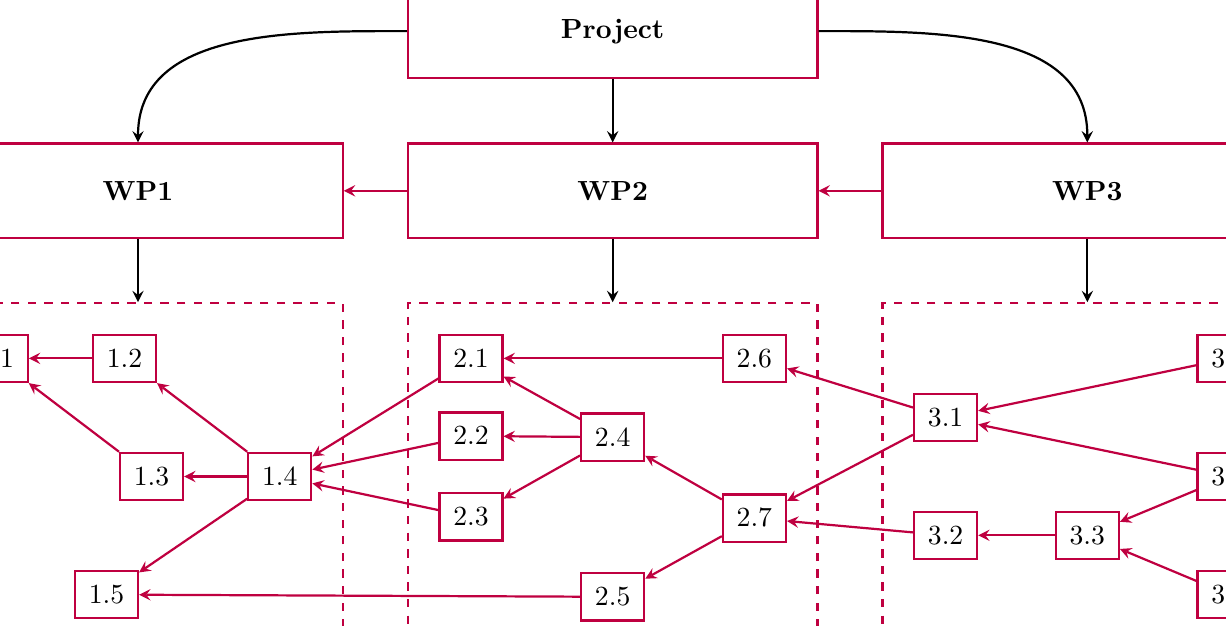
\begin{tikzpicture}[remember picture]
      \newcommand{\wpwidth}[0]{5.2cm}
      \newcommand{\taskheight}[0]{6mm}
      \newcommand{\spacing}[0]{4mm}
      \newcommand{\xspacing}[0]{(2*\spacing+0mm)}
      \newcommand{\yspacing}[0]{(2*\spacing+0mm)}
      \newcommand{\groupheight}[0]{(5*\spacing+4*\taskheight)}
      
      \coordinate (origo) at (0,0);
      
      \tikzstyle{node}=[
        overlay,
        rectangle,
        draw=purple,
        anchor=center,
        align=center,
        thick,
        minimum width=\wpwidth,
        minimum height=1.2cm,
      ]
      \tikzstyle{wp} = [
        node,
      ]
      \tikzstyle{task} = [
        node,
        minimum width=8mm,
        minimum height=\taskheight,
      ]
      \tikzstyle{group} = [
        node,
        dashed,
        minimum width=\wpwidth,
        minimum height=\groupheight,
      ]
      \tikzstyle{phase} = [
        anchor=south,
        align=center,
      ]
      \tikzstyle{dep} = [
        thick,
        ->,
        >=stealth,
        draw=purple,
      ]
      \tikzstyle{edge} = [
        thick,
        ->,
        >=stealth,
        draw,
      ]
      
      % project
      \node[wp] (project) at (origo) {\textbf{Project}};
      
      % intermediary layer
      {
        \node[wp,anchor=north] (wpII) at ([yshift=-\yspacing] project.south) {\textbf{WP2}};
        \node[wp,anchor=east] (wpI) at ([xshift=-\xspacing] wpII.west) {\textbf{WP1}};
        \node[wp,anchor=west] (wpIII) at ([xshift=\xspacing] wpII.east) {\textbf{WP3}};
        
        \draw[dep] (wpII) -- (wpI);
        \draw[dep] (wpIII) -- (wpII);
        
        \draw[edge] (project) to [out=180,in=90] (wpI);
        \draw[edge] (project) to [out=270,in=90] (wpII);
        \draw[edge] (project) to [out=  0,in=90] (wpIII);
      }
      
      % final layer: left group
      {
        \node[group,anchor=north] (gI) at ([yshift=-\yspacing] wpI.south) {};
        
        \node[task,anchor=north west] (gInI)
          at ([yshift=-1*\spacing, xshift=\spacing] gI.north west) {1.1};
        \node[task,anchor=west] (gInII)
          at ([xshift=\xspacing] gInI.east) {1.2};
        \node[task,anchor=east] (gInIV)
          at ([xshift=-\spacing] gI.east) {1.4};
        \node[task,anchor=east] (gInIII)
          at ([xshift=-\xspacing] gInIV.west) {1.3};
        \node[task,anchor=south] (gInV)
          at ([yshift=1*\spacing, xshift=-\spacing] gI.south) {1.5};
        
        \draw[dep] (gInII)  -- (gInI);
        \draw[dep] (gInIII) -- (gInI);
        \draw[dep] (gInIV)  -- (gInII);
        \draw[dep] (gInIV)  -- (gInIII);
        \draw[dep] (gInIV)  -- (gInV);
        
        \draw[edge] (wpI) to [out=270,in=90] (gI);
      }
      
      % final layer: middle group
      {
        \node[group,anchor=north] (gII) at ([yshift=-\yspacing] wpII.south) {};
        
        \node[task,anchor=north west] (gIInI)
          at ([yshift=-1*\spacing, xshift=\spacing] gII.north west) {2.1};
        \node[task,anchor=south west] (gIInII)
          at ([yshift=0.5*\spacing, xshift=\spacing] gII.west) {2.2};
        \node[task,anchor=north west] (gIInIII)
          at ([yshift=-0.5*\spacing, xshift=\spacing] gII.west) {2.3};
        \node[task,anchor=north] (gIInIV)
          at ([yshift=-2*\spacing-\taskheight] gII.north) {2.4};
        \node[task,anchor=north west] (gIInV)
          at ([yshift=-2*\spacing-\taskheight] gIInIV.south west) {2.5};
        \node[task,anchor=north east] (gIInVI)
          at ([yshift=-1*\spacing, xshift=-\spacing] gII.north east) {2.6};
        \node[task,anchor=north west] (gIInVII)
          at ([yshift=-2*\spacing-\taskheight] gIInVI.south west) {2.7};
        
        \draw[dep] (gIInIV) -- (gIInI);
        \draw[dep] (gIInIV) -- (gIInII);
        \draw[dep] (gIInIV) -- (gIInIII);
        \draw[dep] (gIInVI) -- (gIInI);
        \draw[dep] (gIInVII) -- (gIInIV);
        \draw[dep] (gIInVII) -- (gIInV);
        
        \draw[edge] (wpII) to [out=270,in=90] (gII);
      }
      
      % final layer: right group
      {
        \node[group,anchor=north] (gIII) at ([yshift=-\yspacing] wpIII.south) {};
        
        \node[task,anchor=west] (gIIInI)
          at ([yshift=-0.3333333*\groupheight, xshift=\spacing] gIII.north west) {3.1};
        \node[task,anchor=west] (gIIInII)
          at ([yshift= 0.3333333*\groupheight, xshift=\spacing] gIII.south west) {3.2};
        \node[task,anchor=center] (gIIInIII)
          at ([yshift= 0.3333333*\groupheight] gIII.south) {3.3};
        \node[task,anchor=north east] (gIIInIV)
          at ([yshift=-\spacing, xshift=-\spacing] gIII.north east) {3.4};
        \node[task,anchor=east] (gIIInV)
          at ([xshift=-\spacing] gIII.east) {3.5};
        \node[task,anchor=south east] (gIIInVI)
          at ([yshift= \spacing, xshift=-\spacing] gIII.south east) {3.6};
        
        \draw[dep] (gIIInIII) -- (gIIInII);
        \draw[dep] (gIIInIV) -- (gIIInI);
        \draw[dep] (gIIInV) -- (gIIInI);
        \draw[dep] (gIIInV) -- (gIIInIII);
        \draw[dep] (gIIInVI) -- (gIIInIII);
        
        \draw[edge] (wpIII) to [out=270,in=90] (gIII);
      }
      
      
      % final layer: interconnects
      \draw[dep] (gIInI)   -- (gInIV);
      \draw[dep] (gIInII)  -- (gInIV);
      \draw[dep] (gIInIII) -- (gInIV);
      \draw[dep] (gIInV)   -- (gInV);
      \draw[dep] (gIIInI)  -- (gIInVI);
      \draw[dep] (gIIInI)  -- (gIInVII);
      \draw[dep] (gIIInII) -- (gIInVII);
    \end{tikzpicture}
  }
\end{center}
